\chapter{Sistema, diseño y desarrollo}
\label{chap:sistemadesarrollado}

En este capítulo se realizará un análisis del sistema desarrollado, mostrando un catálogo de requisitos que contendrá los requerimientos funcionales y no funcionales de la aplicación.
Después, se describirá el diseño de la herramienta, así como el de cada  uno  de  sus módulos haciendo hincapié en las dependencias propias a cada uno, así como la base de datos utilizada, ó librerías necesarias para su correcto funcionamiento.

\section{Catálogo de requisitos}

A continuación se muestra cada uno de los requisitos funcionales y no funcionales del sistema. Éste apartado está seccionado por los distintos módulos del sistema.

\subsection{Requisitos funcionales}
\subsubsection{Requisitos generales del sistema}
\begin{adjustwidth}{0.5cm}{}
\textbf{Requisito Funcional \#1: No habrá problemas de dependencias.}\\
La herramienta podrá ser ejecutada sin que el usuario final necesite instalar librerías extra (más allá del servicio Tor).\\
\linebreak
\textbf{Requisito Funcional \#2: Las funciones de la aplicación podrán ser lanzadas mediante una interfaz por \textit{shell}.}\\
Esta interfaz requerirá que el usuario seleccione la opción que desea realizar. Por lo tanto, requiere que el usuario interaccione con el sistema.\\	
\linebreak
\textbf{Requisito Funcional \#3: Las funciones de la aplicación podrán ser lanzadas mediante un \textit{script} por consola.}\\
El usuario hará uso de los argumentos a la hora de lanzar el programa para que este ejecute automáticamente, no haciendo necesaria la interacción con el usuario(excepto en aquellos módulos cuya funcionalidad requiera realizar acciones con el mismo).\\
\linebreak
\end{adjustwidth}
\subsubsection{Requisitos de la funcionalidad de \textit{mailing}}
\begin{adjustwidth}{0.5cm}{}
	\textbf{Requisito Funcional \#4: El usuario podrá hacer uso de un \textit{remailer} para enviar e-mails.}\\
	El remailer~\cite{article:remailer} \textit{Mixmaster} podrá ser lanzada directamente desde la herramienta, el cual permitirá al usuario enviar e-mails \textbf{anónimos}.\\
	\linebreak
	\textbf{Requisito Funcional \#5: El usuario podrá enviar e-mails a través de un servicio de e-mails anónimos.}\\
	Este servicio permite enviar correos directamente desde consola, haciendo uso del servicio \textbf{Anonemail de Anonymouse}. \\
	\linebreak
	\textbf{Requisito Funcional \#6: El usuario podrá realizar una ofuscación de estilometría en el envío de e-mails.}\\
	En el emisor de correos anónimos, el usuario tiene la opción de poder ofuscar su texto, aplicando una doble traducción en el cuerpo del mensaje.\\
	\linebreak
	\textbf{Requisito Funcional \#7: El usuario tiene disponible una bandeja de entrada temporal por consola.}\\
	Ésta opción permite al usuario hacer uso del servicio online de https://tempail.com para visualizar, directamente por consola y en tiempo real, los e-mails que van llegando.\\
	\linebreak	
	\textbf{Requisito Funcional \#8: El usuario tiene disponible una bandeja de entrada temporal visible en un navegador.}\\
	Esta opción abre una instancia del navegador Firefox, donde se puede visualizar en tiempo real los correos entrantes mediante el servicio de bandeja temporal https://temptami.com.\\	
\end{adjustwidth}
\subsubsection{Requisitos de la funcionalidad de \textit{accounts}}
\begin{adjustwidth}{0.5cm}{}
	\textbf{Requisito Funcional \#9: El usuario podrá crear automáticamente cuentas de usuario en Facebook.}\\
	Ésta opción automatiza el proceso de registro en la red social Facebook, y logra generar un nombre y apellidos válidos, así como realizar una confirmación de la cuenta mediante correo electrónico(haciendo uso de la bandeja temporal vista en el Requisito Funcional \#8).\\
	\linebreak
	\textbf{Requisito Funcional \#10: El usuario podrá loguear automáticamente un usuario ya registrado en Facebook.}\\
	Este servicio automatiza el proceso de inicio de sesión de un usuario \textbf{(el cual debe haber sido registrado previamente)} en la red social Facebook. \\
	\linebreak
	\textbf{Requisito Funcional \11: El usuario podrá crear automáticamente cuentas de usuario en Instagram.}\\
	Ésta opción automatiza el proceso de registro en la red social Facebook, y logra generar un nombre de usuario y contraseña válidos, así como un correo electrónico temporal con el que registrarse(en este caso no es necesario realizar una confirmación de cuenta mediante correo).\\
	\linebreak
	\textbf{Requisito Funcional \#11: El usuario podrá loguear automáticamente un usuario ya registrado en Instagram.}\\
	Este servicio automatiza el proceso de inicio de sesión de un usuario \textbf{(el cual debe haber sido registrado previamente)} en la red social Instagram. \\
	\linebreak	
	\textbf{Requisito Funcional \#12: El usuario podrá realizar una acción automática en Instagram una vez realizado el inicio de sesión.}\\
	Ésta opción, a modo de ejemplo, permite seguir a una persona y, en el caso de que tenga un perfil público, realizar la acción "Me gusta" a algunas de sus fotos. \\
	\linebreak		
	\textbf{Requisito Funcional \#13: El usuario podrá crear automáticamente cuentas de usuario en un periódico on-line.}\\
	Este requisito implica automatizar el proceso de registro, con su correspondiente confirmación de correo, en la web de un periódico on-line. \\
	\linebreak
	\textbf{Requisito Funcional \#14: El usuario podrá loguearse con una cuentas de usuario ya creada en un periódico on-line.}\\
	Ésta opción permite, una vez realizado al menos un registro en la web, realizar un inicio de sesión con un usuario registrado. \\
	\linebreak				
	\textbf{Requisito Funcional \#15: El usuario podrá realizar comentarios en noticias recientes una vez realizado un inicio de sesión.}\\
	En este caso, se le brinda al usuario la opción de visualizar los titulares de las noticias recientes con más comentarios, así como realizar comentarios en ellas, \textbf{todo ello mediante consola}. \\
	\linebreak			
	\textbf{Requisito Funcional \#16: El usuario podrá realizar comentarios en noticias recientes una vez realizado un inicio de sesión.}\\
	En este caso, se le brinda al usuario la opción de visualizar los titulares de las noticias recientes con más comentarios, así como realizar comentarios en ellas, \textbf{todo ello mediante consola}. \\
	\linebreak	
	\textbf{Requisito Funcional \#17: El usuario podrá loguearse con una cuentas de usuario ya creada en un periódico on-line.}\\
	Ésta opción permite, una vez realizado al menos un registro en la web, realizar un inicio de sesión con un usuario registrado. \\
	\linebreak				
	\textbf{Requisito Funcional \#18: El usuario podrá realizar comentarios en noticias recientes una vez realizado un inicio de sesión.}\\
	En este caso, se le brinda al usuario la opción de visualizar los titulares de las noticias recientes con más comentarios, así como realizar comentarios en ellas, \textbf{todo ello mediante consola}. \\
	\linebreak			
	\textbf{Requisito Funcional \#19: El usuario podrá realizar comentarios en noticias recientes una vez realizado un inicio de sesión.}\\
	En este caso, se le brinda al usuario la opción de visualizar los titulares de las noticias recientes con más comentarios, así como realizar comentarios en ellas, \textbf{todo ello mediante consola}. \\
	\linebreak	
	\textbf{Requisito Funcional \#20: El usuario podrá realizar comentarios en noticias recientes una vez realizado un inicio de sesión.}\\
	En este caso, se le brinda al usuario la opción de visualizar los titulares de las noticias recientes con más comentarios, así como realizar comentarios en ellas, \textbf{todo ello mediante consola}. \\
	\linebreak	
	\textbf{Requisito Funcional \#21: El usuario podrá realizar comentarios en noticias recientes una vez realizado un inicio de sesión.}\\
	En este caso, se le brinda al usuario la opción de visualizar los titulares de las noticias recientes con más comentarios, así como realizar comentarios en ellas, \textbf{todo ello mediante consola}. \\
	\linebreak	
	\textbf{Requisito Funcional \#22: El usuario podrá realizar comentarios en noticias recientes una vez realizado un inicio de sesión.}\\
	En este caso, se le brinda al usuario la opción de visualizar los titulares de las noticias recientes con más comentarios, así como realizar comentarios en ellas, \textbf{todo ello mediante consola}. \\				
	\linebreak		
	\textbf{Requisito Funcional \#23: El usuario podrá registrar un usuario en un foro de discusión.}\\
	Éste servicio automatiza el proceos de registro de un usuario en un foro de discusión. En este caso, automatiza la confirmación por correo, \textbf{además de resolver un pequeño captcha} que solicita la página al registrarse. \\
	\linebreak	
	\textbf{Requisito Funcional \#24: El usuario podrá loguearse con una cuenta ya creada en un foro de discusión.}\\
	Este requisito automatiza el hecho de realizar un inicio de sesión la página web de un foro de discusión, previo registro. \\
	\linebreak	
	\textbf{Requisito Funcional \#25: El usuario puede realizar comentarios en diversos temas de un foro de discusión.}\\
	El servicio permite al usuario elegir el tema sobre el que realizar un comentario. Tras ello, aparecen los \textit{post} más destacados, donde también se le brinda al usuario la opción de comentar, \textbf{todo ello mediante consola}.\\			
	\linebreak		
	\textbf{Requisito Funcional \#26: El usuario puede elegir el navegador utilizado para las tareas automáticas.}\\
	El usuario tiene a disposición elegir entre un navegador Firefox normal y un navegador que haga uso de \textbf{Tor}(para mayor grado de anonimato).\\				
\end{adjustwidth}
\subsubsection{Requisitos de la funcionalidad relativos a la base de datos}
\begin{adjustwidth}{0.5cm}{}
	\textbf{Requisito Funcional \#27: El sistema podrá crear una base de datos.}\\
	En el primer uso de la herramienta con la funcionalidad de \textit{accounts}, el sistema creará una base de datos \textbf{SQLite encriptada mediante el algoritmo AES de 256 bits} para almacenar a los usuarios de diversas páginas. \\
	\linebreak		
	\textbf{Requisito Funcional \#28: El sistema podrá crear tablas en la base de datos.}\\
	El sistema podrá crear varias tablas en la base de datos, una por cada una de las páginas en las que se pueden realizar acciones de registro y logueo de usuarios. \\
	\linebreak		
	\textbf{Requisito Funcional \#29: El sistema podrá insertar tuplas.}\\
	El sistema insertará los usuarios registrados en cada una de las páginas a la tabla que corresponda de la base de datos. \\	
	\linebreak			
\end{adjustwidth}
\subsection{Requisitos no funcionales}
\begin{adjustwidth}{0.5cm}{}
	\textbf{Requisito No Funcional \#1: El sistema será de código libre y abierto.}\\
	Cualquier usuario podrá editar y/o modificar cualquier aspecto de la aplicación. para ello se proporcionará en el manual de usuario un enlace al repositorio de GitHub donde se encuentra el proyecto. \\
	\linebreak		
	\textbf{Requisito No Funcional \#2: El código será modular.}\\
	Se facilitará en la medida de lo posible la inclusión de nuevas funcionalidades a la herramienta, haciendo uso de un código modular que no requiera realizar grandes cambios en el resto del programa. \\
	\linebreak		
	\textbf{Requisito No Funcional \#3: El código contendrá comentarios.}\\
	Cada una de las funciones del código estará documentada, explicando su funcionamiento. \\	
	\linebreak			
	\textbf{Requisito No Funcional \#4: El sistema no hará uso de permisos superusuario.}\\
	La herramienta no requerirá ser un usuario con privilegios para poder usarse. \\	
	\linebreak
	\textbf{Requisito No Funcional \#5: El sistema deberá ejecutar las tareas de forma rápida y eficiente.}\\
	Cualquier tarea ejecutada por el sistema (ya sea dada de alta de usuarios, inicio de sesión, envío de e-mails ó posteo de comentarios) no deberá demorarse en exceso, con un tiempo límite de 2 minutos por tarea. \\		
\end{adjustwidth}
\newpage
\section{Diseño del sistema}

Esta sección se encarga de explicar al detalle las decisiones de diseño tomadas, así como la arquitectura final del sistema. 

La herramienta, cuyo objetivo es el de facilitar al usuario el realizar tareas básicas manteniendo siempre la premisa de un buen anonimato, así como la automatización de ciertos procesos, ha sido diseñada en lenguaje Python. 

Se ha elegido Python (en su versión 2.7) puesto que la gran mayoría de herramientas de auditoría han sido diseñadas en este lenguaje, y es posible reutilizar código así como importar librerías muy útiles en el campo de la seguridad informática.

El desarrollo en Python, además, simplifica la codificación debido a su sencilla sintaxis, muy próxima al simple pseudocódigo. Además, puesto que el orden de tiempo para ejecutar las tareas depende en gran medida de las respuestas web y no tanto de la eficiencia del lenguaje, no se ha considerado el hecho de utilizar un lenguaje de más bajo nivel.

La programación del proyecto ha sido elaborada en un entorno Linux, concretamente en una distribución Ubuntu, y únicamente ha sido probada en este sistema operativo.

En todo el proyecto se ha seguido un proceso de \textit{web-scraping}~\cite{article:webscraping} (utilizando distintas librerías) para poder utilizar los servicios de un sitio web de forma \textbf{sencilla, por consola, rápida y automática en la gran parte de los casos.}

En esta aplicación se han tenido en cuenta dos modos de ejecución. 

\begin{itemize}
	\item \textbf{Script}: En este modo el programa recibirá argumentos con los que se lanzará automáticamente la funcionalidad deseada, sin pasar por un menú de selección.
	\item \textbf{Interfaz}: Si optamos por un menú interactivo, se preguntará al usuario qué acción realizar, de forma que el usuario decide en tiempo real qué opción seleccionar.
\end{itemize}

\subsection{Diseño de la sección de \textit{mailing}}

La funcionalidad de mailing la podemos dividir en los módulos en los que está compuesta. 

El \textbf{módulo de envío de correos anónimo} se encarga de la extracción de información de la página \textbf{http://anonymouse.org/anonemail.html}. La extracción de información se realiza mediante el uso de la librería \textbf{\textit{mechanize}}. Ésta potente librería disponible en Python se utiliza para automatizar información con páginas web. Automáticamente almacena y envía \textit{cookies}, permite redirecciones web y puede \textbf{interactuar y enviar formularios}(lo que nos permite el envío de correos por medio de esta página).
Se ha incluido una modificación en las \textit{headers} del navegador, para tratar de evitar el traceo de identidad.

También se ha añadido la posibilidad de realizar un proceso de \textbf{ofuscación de estilometría} rápido y simple. Para ello se hace uso del ofuscador disponible en la página https://skaillz.net/obfuscator/. La ofuscación se realiza mediante un doble proceso de traducción automático. 
Ésta opción está disponible en el cuerpo del mensaje/correo.

La interfaz al uso es la siguiente:

\begin{figure}[H]
	\centering
	\begin{subfigure}{0.5\textwidth}
		\centering
		\mbox{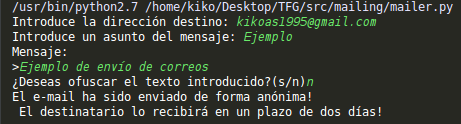
\includegraphics[width=3.50in]{images/sin_ofuscar.png}}
		\caption{Mensaje enviado}
		\label{fig:sub1}
	\end{subfigure}%
	\begin{subfigure}{0.5\textwidth}
		\centering
		\mbox{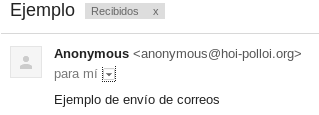
\includegraphics[width=2.75in]{images/recibido_sin.png}}
		\caption{Mensaje recibido}
		\label{fig:sub2}
	\end{subfigure}
	\caption{Ejemplo de uso sin ofuscar el cuerpo de texto}
	\label{fig:mailer}
\end{figure}

\begin{figure}[H]
	\centering
	\begin{subfigure}{0.5\textwidth}
		\centering
		\mbox{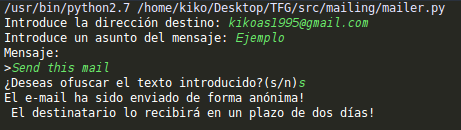
\includegraphics[width=3.50in]{images/con_ofuscar.png}}
		\caption{Mensaje enviado}
		\label{fig:sub1}
	\end{subfigure}%
	\begin{subfigure}{0.5\textwidth}
		\centering
		\mbox{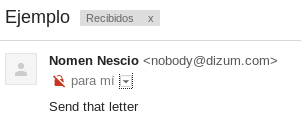
\includegraphics[width=2.6in]{images/recibido_con.png}}
		\caption{Mensaje recibido}
		\label{fig:sub2}
	\end{subfigure}
	\caption{Ejemplo de uso ofuscando el cuerpo de texto}
	\label{fig:mailer}
\end{figure}

Debido a la cola de mensajes de la página, el envío se puede llegar a demorar bastante, así que el destinatario recibirá el correo en un intervalo de \textbf{24-48} horas.

En cuanto a bandejas de entrada volátiles, se han implementado \textbf{dos}. El motivo es que muchas de las páginas utilizadas en la sección de \textit{accounts} bloqueaban alguna de las dos, así que convenía tener una alternativa.

En la \textbf{primera} se hace uso de la página https://tempail.com/ para poder visualizar los correos entrantes en tiempo real directamente desde la interfaz del programa. Se hizo uso de las librerías \textbf{requests} y \textbf{html} para lograr la funcionalidad deseada. A continuación una captura de la bandeja de entrada en funcionamiento:

\begin{figure}[H]
	\centerline{
		\mbox{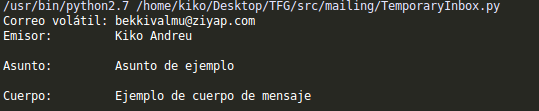
\includegraphics[width=4.00in]{images/inbox1.png}}
	}
	\caption{Ejemplo de bandeja de entrada}
	\label{fig:tempail_inbox}
\end{figure}

La otra bandeja de entrada volátil hace uso de la web https://temptami.com/, un servicio de bandeja de entrada temporal algo menos conocido que tempail y, por ende, con menos restricciones para el uso en registros de diversas páginas como FaceBook. A diferencia de los anteriores módulos, esta página hace necesario realizar \textit{web-scraping} teniendo en cuenta código JavaScript. Es por ello que la librería para examinar la página ahora es \textbf{Selenium}, una librería que provee al usuario de automatización de procesos en páginas web, mediante un \textbf{WebDriver}, que es el nombre de la interfaz donde se ejecutan dichos procesos. 

La bandeja de entrada temporal del servicio \textbf{TempTami}, por ende, tiene como objetivo principal la validación de \textbf{correos de confirmación} para el registro en varias páginas web, que veremos en el apartado siguiente. 

Por ello, el uso que se le da es bastante distinto al de la primera bandeja mencionada.

\subsection{Diseño de la sección de \textit{accounts}}

Es la sección con mayor trabajo de la aplicación. El objetivo de esta sección es automatizar \textbf{procesos de registro e inicio de sesión en diversas páginas web.}
Para ello se ha optado por el uso de una clase abstracta \textbf{"Bot"}, la cual contiene las funciones \textbf{signup} y \textbf{login}.

Todos y cada uno de los módulos relativos a la generación de cuentas anónimas \textbf{heredan} dicha clase abstracta. Por tanto, cada uno de ellos implementa como mínimo una función de registro y otra de inicio de sesión en una página web, \textbf{pero hay ciertos módulos que cuentan con funcionalidades extra}, como el caso del módulo \textbf{instagram.py}, que cuenta con una función para seguir a un usuario y dar "Me gusta" a sus publicaciones. 

Se han implementado módulos de creación y uso de cuentas automáticas en diversas páginas como:

\begin{itemize}
	\item Redes sociales (Facebook e Instagram)
	\item Un periódico online (con funcionalidad para visualizar titulares de las noticias directamente desde consola, así como realizar comentarios en ellas).
	\item Un foro de discusión (con funcionalidad para visualizarlos temas de discusión más recientes directamente desde consola, así como realizar comentarios en ellos).
	\item Una plataforma web sobre medidas políticas (con funcionalidad para apoyar automáticamente las medidas más recientes).
\end{itemize}

Como se ha comentado en el capítulo anterior, para el registro de varias de las páginas implementadas se debe hacer uso de una bandeja de entrada temporal para la confirmación de e-mails de verificación.
 
Asimismo, se ha procurado lidiar con problemas como \textbf{captchas} para comprobar si el usuario es humano(se ha conseguido "\textit{saltar}" el captcha en el registro del foro de discusión. No obstante otros más complejos como los captchas de reconocimiento de letras, aun con el uso de librerías enfocadas en ellos, no obtienen buen índice de acierto). 

Es importante recalcar cómo funciona el sistema de \textbf{cuentas}. En el momento que se lanza la función de \textbf{registro} en cualquiera de las páginas implementadas, la herramienta guarda al usuario registrado en una tabla de la base de datos dedicada a esa página. Con ello, se logra realizar un inicio de sesión \textbf{extrayendo un usuario ya registrado de la tabla de la base de datos}. Todo ello es realizado de forma automática, sin que el usuario necesite hacer uso de dicha base de datos intencionadamente.

Todos estos módulos han sido implementados usando la librería \textbf{Selenium}, debido a la existencia de código JavaScript en prácticamente todas las páginas estudiadas. 

Cabe destacar que las \textbf{páginas grandes} como Facebook e Instagram, restringen el número de registros en un tiempo determinado \textbf{usando la misma IP.} Es por esto que se ha considerado dar a elegir entre el uso de dos \textbf{WebDrivers}. 

\begin{itemize}
	\item El primero basado en un navegador \textbf{Firefox} con una configuración por defecto.
	\item El segundo basado en un navegador Firefox con un proxy Tor habilitado (\textbf{Tor Browser}).
\end{itemize} 

Mientras que el uso del WebDriver de Firefox con configuración por defecto agiliza los procesos de registro e inicio de sesión con una velocidad más que aceptable(del orden de menos de\textbf{ dos minutos} para el registro e inicio de sesión completos), el navegador \textbf{Tor Browser} impide que páginas como Facebook ó Instagram restrinjan el número de registros tan fácilmente, aumentando además nuestro nivel de \textbf{privacidad y anonimato}.

\subsection{Diseño de la base de datos de \textit{accounts}}

La herramienta contiene un módulo dedicado a la implementación de una base de datos \textbf{SQLite }que, además, \textbf{está cifrada}.

El encriptación, la cual usa un esquema AES de 256 bit transparente al usuario, se consigue mediante el uso de la librería \textbf{pysqlcipher}.

El módulo dedicado a la base de datos, contiene varias funciones para el manejo de la misma. Dichas funciones son llamadas desde los módulos de la sección de \textbf{accounts}. Entre ellas hay funciones para la inserción de tuplas(con creación automática de la tabla en el caso de que no exista), consultas para obtener una tupla concreta ó aleatoria.

La base de datos que se crea contiene tantas tablas como páginas en las que se ha implementado un registro de usuarios, y todas ellas tendrán la misma estructura, contando con campos como \textbf{username registrado, contraseña y e-mail de registro.}

\begin{table}[H]
	\centering
	\label{my-label}
	\begin{tabular}{|c|c|c|c|}
		\hline
		\rowcolor[HTML]{BBDAFF} 
		\multicolumn{4}{|c|}{\cellcolor[HTML]{BBDAFF}'facebook'} \\ \hline
		\rowcolor[HTML]{ECF4FF} 
		\textbf{integer} 'id'    & \textbf{text} 'usr'   & \textbf{text} 'pwd'   & \textbf{text} 'email'   \\ \hline
	\end{tabular}
	\caption{Ejemplo de tabla del sistema}
\end{table}

\section{Implementación, desarrollo y pruebas}
\subsection{Librerías utilizadas}

La herramienta desarrollada hace uso de las siguientes librerías:

\begin{itemize}
	\item \textbf{mechanize}: Para la implementación del módulo de envío de e-mails.
	\item \textbf{requests}: Utilizado en la primera bandeja de entrada temporal para interacción con la página web.
	\item \textbf{lxml}: Utilizado principalmente para el parseo de un elemento HTML en un objeto XML.
	\item \textbf{re}: Librería que permite el manejo de expresiones regulares. Es utilizado para la validación de e-mails de confirmación.
	\item \textbf{selenium}: Librería que brinda la posibilidad de automatizar procesos utilizando \textbf{WebDrivers}.
	\item \textbf{tbselenium}: Librería que permite el uso del navegador Tor Browser como WebDriver de selenium.	
	\item \textbf{pysqlcipher}: Librería utilizada para el manejo de la base de datos SQLite encriptada.	
	\item \textbf{mixmaster}: Remailer utilizado en la sección de \textit{mailing}.
	\item \textbf{names}: Librería que genera nombres y apellidos aleatorios.	Es utilizada para el registro de cuentas automático.
\end{itemize}

Además de estas, se ha realizado un estudio de la red Tor, así como sus servicios ocultos, donde se han utilizado las siguientes librerías:
\begin{itemize}
	\item \textbf{Tortazo}: Herramienta con la que es posible realizar auditorías de servicios ocultos en Tor, así como recopilación de información de nodos de salida.
	\item \textbf{stem}: Stem permite controlar una instancia Tor desde Python, así como la creación de un servicio oculto.
	\item \textbf{Flask}: Framework ligero utilizado para la creación de servicios, en este caso enfocado a la red Tor.
\end{itemize}
\subsection{Desarrollo}

El desarrollo de la herramienta comenzó con el módulo main interactivo, como base desde el que se lanzarían el resto de módulos Python.

Tras ello, se prosigiuió con el desarrollo de los módulos incluidos en el paquete \textbf{mailing}. Estos son:
\begin{itemize}
	\item \textbf{mailer.py}: Contiene la funcionalidad de envío de correos anónimos. Como extra se añade la posibilidad de ofuscar el contenidos del correo a enviar mediante un módulo llamado \textbf{obfuscator.py}, el cual realiza una ofuscación estilométrica rápida y eficaz.
	\item \textbf{TemporaryInbox1.py}: Contiene la bandeja de entrada temporal en tiempo real.
	\item \textbf{TemporaryInbox2.py}: Contiene la funcionalidad de verificación de e-mails de confirmación para el registro de cuentas(haciendo uso de una bandeja de entrada temporal).
\end{itemize}

Una vez finalizada la sección de \textit{mailing}, se realizó el paquete \textit{db}, el cual contiene el módulo \textbf{criptodb.py}, que sería utilizado para la funcionalidad del paquete de \textit{accounts}.
Dicho paquete cuenta con módulos relativos a la automatización de registro e inicio de sesión en diversas páginas, así como el módulo de la clase abstracta \textbf{Bot.py} la cual es heredada por los módulos anteriormente mencionados. Entre ellos encontramos:

\begin{itemize}
	\item \textbf{Facebook.py}: Contiene la funcionalidad de registro e inicio de sesión automático en la red social Facebook.
	\item \textbf{Instagram.py}: Contiene la funcionalidad de registro e inicio de sesión automático en la red social Instagram.
	\item \textbf{osoigo.py}: Contiene la funcionalidad de registro e inicio de sesión automático en un portal sobre apoyo de medidas políticas, así como una funcionalidad automática de apoyo a propuestas.
	\item \textbf{eldiario.py}: Contiene la funcionalidad de registro e inicio de sesión automático en un periódico \textit{online}, así como la visualización de los titulares más comentados recientemente, con la posibilidad de enviar comentarios desde la interfaz en consola Python directamente.
	\item \textbf{scenebeta.py}: Contiene la funcionalidad de registro e inicio de sesión automático en un foro de discusión, así como la visualización de los \textit{posts} más recientes, con la posibilidad de enviar comentarios a dichos \textit{posts} desde la interfaz en consola Python directamente.
\end{itemize}